% Chapter 5

\chapter{Results and discussion} % Main chapter title

\label{Chapter5} % For referencing the chapter elsewhere, use \ref{Chapter5} 
\subsection{Small Network solved by D-Wave Quantum Annealer}
\begin{figure}[H]
  \begin{center}
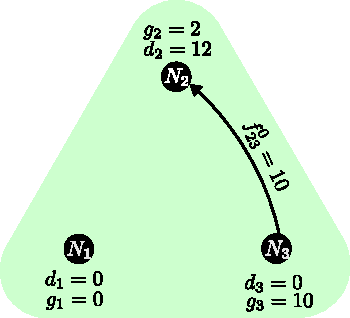
\includegraphics[width=0.4\textwidth]{Figures/Green_Final.pdf}
  \end{center}
  \caption{Graphical solution of three node problem.}
  \label{fig: Green_final}
\end{figure}
 \begin{table}[H]
\centering
\begin{tabular}{ |c|c|c|c|c|c|c|c| }
  \hline			
  $\mathbf{x_{12}}$ & $\mathbf{x_{13}}$ & $\mathbf{x_{23}}$ & $\mathbf{g_{1}}$ & $\mathbf{g_{2}}$ & $\mathbf{g_{3}}$ & \textbf{Energy} & \textbf{Feasible} \\
  \hline
    0 & 0 & 1 & 0 & 2 & 10 & 60 & True \\
  \hline
    0 & 0 & 1 & 0 & 3 & 9 & 63 & True \\
  \hline
    0 & 0 & 1 & 0 & 4 & 8 & 66 & True \\
  \hline
    0 & 0 & 1 & 0 & 6 & 7 & 69 & True \\
  \hline
\end{tabular}
\caption{D-Wave's feasible solutions to the TEP combinatorial optimization problem.}
\label{tab:SmallNetworkResults}
\end{table}
\subsection{Hybrid Approaches of D-Wave}
